\section{Task 2: a national trend map}\label{sec:q2}

\subsection{Design}

For each of the 25 cities we compute the same annual indices as in Section~\ref{sec:q1} and test the same five trends. Five hypotheses on 25 cities is 125 tests, and at a nominal 5\% level roughly six would be significant by chance alone. Reporting those six as ``trends'' is the most common error in this literature, so we control the false discovery rate with the Benjamini--Hochberg procedure \cite{bh1995} and report only discoveries with $q\le0.05$. Because the six indices are tested on the same 25 series we pool them into one family: five indices over 25 cities plus the threshold count over the 21 cities where it is defined, i.e.\ 146 finite tests. Controlling each index separately over its own cities would be less conservative and would return 1, 1, 1, 11 and 13 discoveries instead of 2, 1, 1, 7 and 9. We report the pooled family, and we also report the median Sen slope, because the median is not distorted by the few cities with very large trends.

\subsection{What actually trends}

The pattern is sharply selective (Table~\ref{tab:q2sig}). Annual totals trend in only two cities, and the one-day maximum in one. In contrast, seven cities have a significant trend in daily intensity and nine in the number of wet days. A national signal that appears in frequency and intensity but not in totals is the spatial analogue of the Zhengzhou result: rainfall is being redistributed within the year rather than increased.

\begin{table}[H]
\centering
\caption{National trend summary, 25 cities, 1961--2020, Benjamini--Hochberg $q\le0.05$.}
\label{tab:q2sig}
\footnotesize
\setlength{\tabcolsep}{4pt}
\begin{tabular}{lrrr}
\toprule
Index & Sig. & Median Sen & Range of Sen\\
\midrule
Total (mm) & 2 & $+3.13$ & $-36.5$ to $+60.5$\\
Rx1day (mm) & 1 & $+1.00$ & $-4.19$ to $+13.51$\\
R95p (mm) & 1 & $-1.01$ & $-22.2$ to $+17.3$\\
SDII (mm\,d$^{-1}$) & 7 & $+0.240$ & $+0.047$ to $+0.867$\\
Wet days (d) & 9 & $-2.50$ & $-10.96$ to $+2.22$\\
Days $\ge50$\,mm (\% dec$^{-1}$) & 0 & $+2.71\%$ & $-15.3\%$ to $+9.1\%$\\
\bottomrule
\end{tabular}
\end{table}

Two entries in Table~\ref{tab:q2sig} deserve emphasis. First, the SDII slope is positive in all 25 cities, with a median of $+0.24$\,mm\,d$^{-1}$ per decade: although only seven are individually significant, the sign is unanimous, which is much stronger evidence than any single test. Second, the threshold-count trends are noisy and none survives FDR control, so we do not claim a national increase in heavy-rain days.

The extremes of the distribution of trends are worth naming. Haikou has the largest increase in Rx1day ($+13.51$\,mm\,dec$^{-1}$, $q=0.23$), Wuhan $+5.83$ ($q=0.29$) and Jinan $+3.51$ ($q=0.46$); Beijing has the largest decrease ($-4.19$\,mm\,dec$^{-1}$, $q=0.23$). Nanning's R95p falls by 22.2\,mm\,dec$^{-1}$, Kunming by 14.2 and Beijing by 15.1. None of these individual slopes survives FDR control except Urumqi's Rx1day increase ($+3.33$\,mm\,dec$^{-1}$, $q<0.01$), which is a reminder that a large slope on a short record is not evidence.

\subsection{Regional structure}

Pooling cities into six belts (North China, Northeast, Yangtze, South, Northwest, Southwest) shows that the sign of the total-rainfall trend is regional, not national: North China $-6.4$\,mm\,dec$^{-1}$, Northeast $+4.6$, Yangtze $+20.2$, South $+21.5$, Northwest $+12.5$, Southwest $-27.1$. Wet-day counts fall in every belt, which is why the national median wet-day slope is negative while the national median total slope is positive. A policy that reads only the national mean would conclude that nothing is happening.

\begin{figure}[H]
\centering
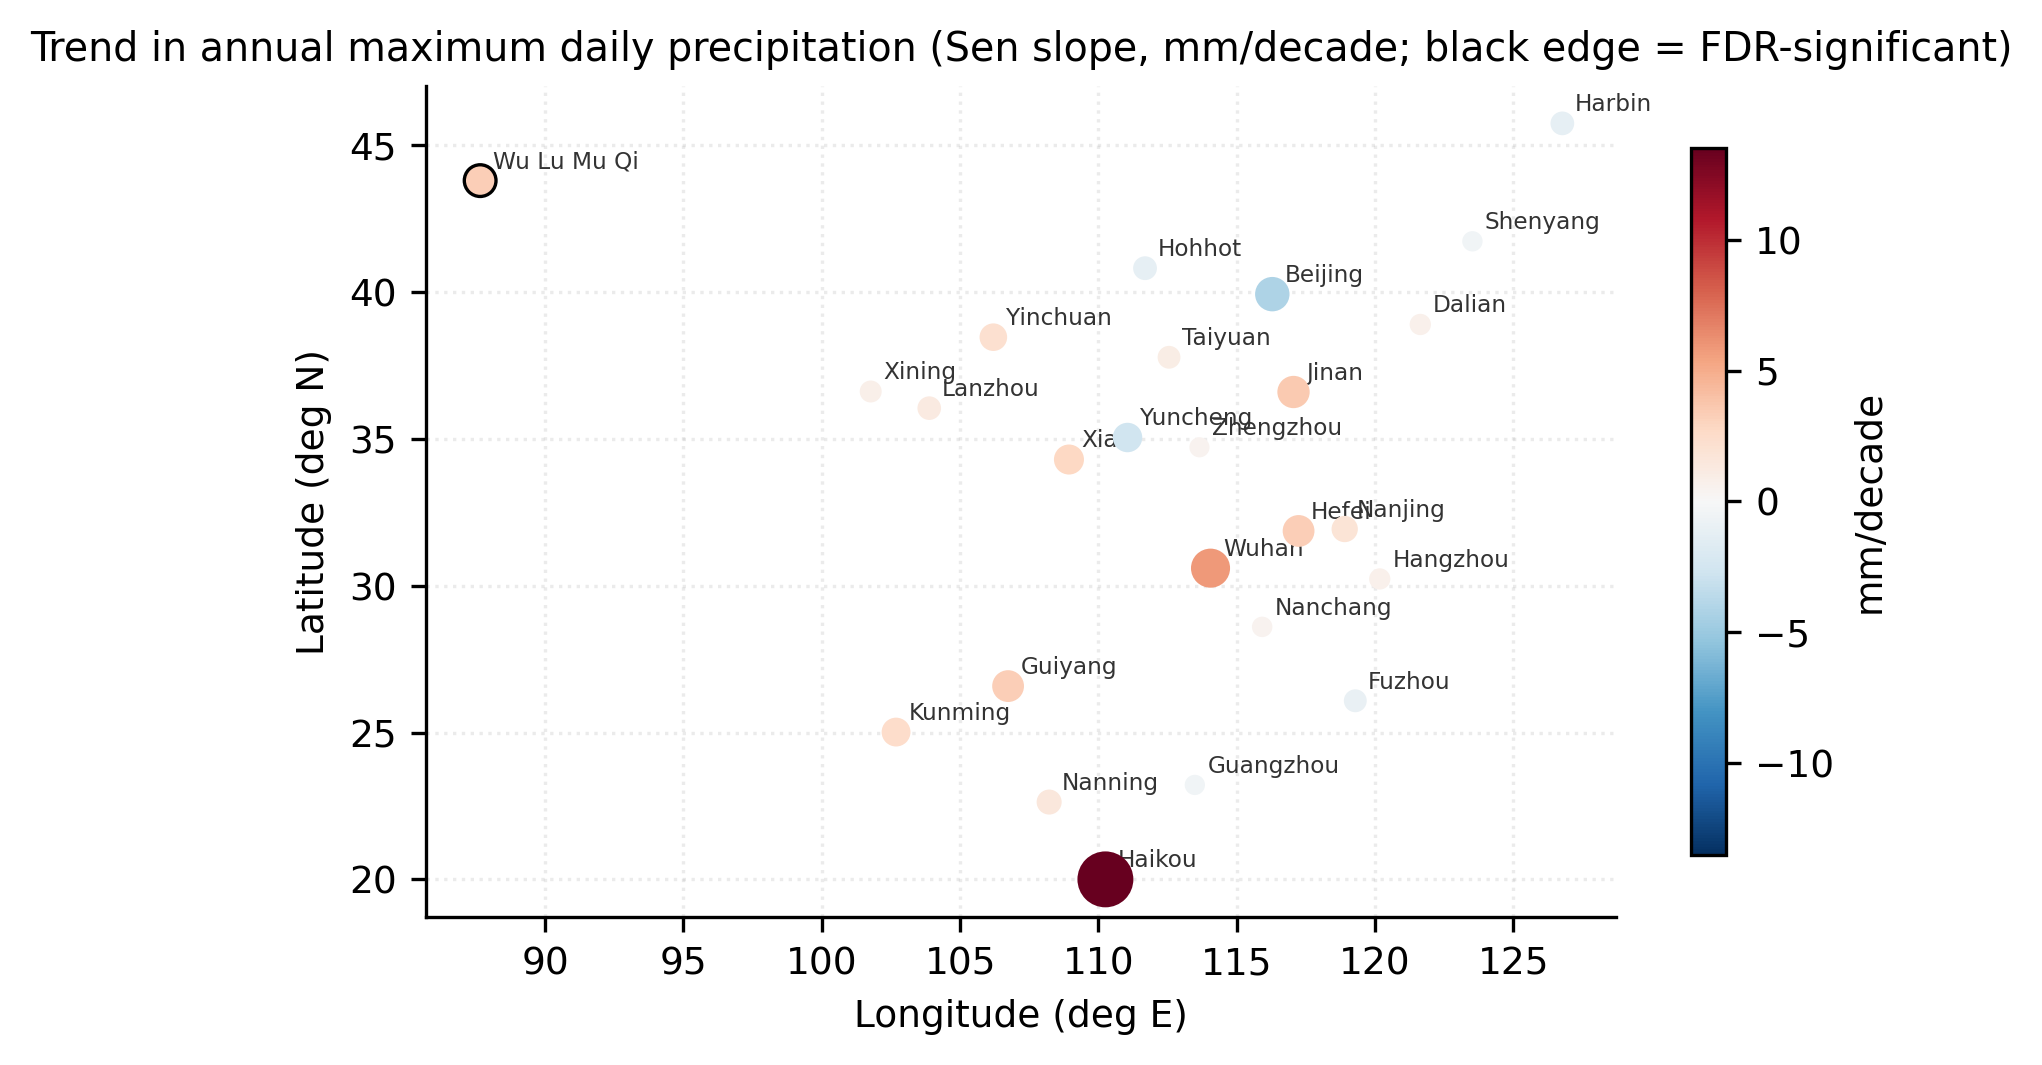
\includegraphics[width=0.38\linewidth]{../02_figures/fig07_trend_map_rx1day.png}
\caption{Sen slope of annual maximum one-day rainfall (mm per decade) for the 25 cities; red denotes increasing extremes and blue decreasing. Circle size scales with the absolute slope.}
\label{fig:maprx}
\end{figure}

\subsection{Classification}

To avoid imposing a geographical partition, we cluster the cities on five standardised trend features (Rx1day, total, R95p, SDII, days $\ge50$\,mm) plus mean intensity, with $k$-means and $k$ chosen by silhouette. The optimum is $k=2$ (silhouette 0.336; $k=3$ gives 0.238), and the two clusters are geographically coherent:

\begin{itemize}[leftmargin=1.4em,itemsep=1pt]
\item \textbf{Cluster 0 (17 cities, continental):} mean annual total 602\,mm and mean Rx1day 63.4\,mm; per decade the Rx1day trend is $+0.80$\,mm, the total trend $-4.66$\,mm, the R95p trend $-4.10$\,mm and the count of days above 50\,mm changes by $-1.85\%$.
\item \textbf{Cluster 1 (8 cities, humid south):} mean annual total 1\,389\,mm and mean Rx1day 113.8\,mm; per decade the Rx1day trend is $+3.03$\,mm, the total trend $+34.2$\,mm, the R95p trend $+4.36$\,mm and the count of days above 50\,mm rises by $+6.49\%$.
\end{itemize}

The split is not a restatement of latitude: it says that the humid south is both wetter and becoming more extreme, whereas the continental interior is drying in total but not becoming less extreme per event. The city-by-index matrix, the cluster geometry and the regional anomaly series are shown in Appendix~\ref{app:extrafig}. This is the input to the risk ranking of Section~\ref{sec:q3}.